%Version 3 December 2023
% See section 11 of the User Manual for version history
%
%%%%%%%%%%%%%%%%%%%%%%%%%%%%%%%%%%%%%%%%%%%%%%%%%%%%%%%%%%%%%%%%%%%%%%
%%                                                                 %%
%% Please do not use \input{...} to include other tex files.       %%
%% Submit your LaTeX manuscript as one .tex document.              %%
%%                                                                 %%
%% All additional figures and files should be attached             %%
%% separately and not embedded in the \TeX\ document itself.       %%
%%                                                                 %%
%%%%%%%%%%%%%%%%%%%%%%%%%%%%%%%%%%%%%%%%%%%%%%%%%%%%%%%%%%%%%%%%%%%%%

%%\documentclass[referee,sn-basic]{sn-jnl}% referee option is meant for double line spacing

%%=======================================================%%
%% to print line numbers in the margin use lineno option %%
%%=======================================================%%

%%\documentclass[lineno,sn-basic]{sn-jnl}% Basic Springer Nature Reference Style/Chemistry Reference Style

%%======================================================%%
%% to compile with pdflatex/xelatex use pdflatex option %%
%%======================================================%%

%%\documentclass[pdflatex,sn-basic]{sn-jnl}% Basic Springer Nature Reference Style/Chemistry Reference Style


%%Note: the following reference styles support Namedate and Numbered referencing. By default the style follows the most common style. To switch between the options you can add or remove “Numbered” in the optional parenthesis. 
%%The option is available for: sn-basic.bst, sn-vancouver.bst, sn-chicago.bst%  
 
%%\documentclass[pdflatex,sn-nature]{sn-jnl}% Style for submissions to Nature Portfolio journals
%%\documentclass[pdflatex,sn-basic]{sn-jnl}% Basic Springer Nature Reference Style/Chemistry Reference Style
%%\documentclass[pdflatex,sn-mathphys-num,lineno]{sn-jnl}% Math and Physical Sciences Numbered Reference Style 
%%\documentclass[pdflatex,sn-mathphys-ay]{sn-jnl}% Math and Physical Sciences Author Year Reference Style
%%\documentclass[pdflatex,sn-aps]{sn-jnl}% American Physical Society (APS) Reference Style
%%\documentclass[pdflatex,sn-vancouver,Numbered]{sn-jnl}% Vancouver Reference Style
%%\documentclass[pdflatex,sn-apa]{sn-jnl}% APA Reference Style 
%%\documentclass[pdflatex,sn-chicago]{sn-jnl}% Chicago-based Humanities Reference Style

\documentclass[pdflatex,sn-mathphys-num,lineno]{sn-jnl}% Math and Physical Sciences Numbered Reference Style 
%%\documentclass[pdflatex,sn-mathphys-num]{sn-jnl}% Math and Physical Sciences Numbered Reference Style 
%%%% Standard Packages
%%<additional latex packages if required can be included here>

\usepackage{graphicx}%
\usepackage{multirow}%
\usepackage{amsmath,amssymb,amsfonts}%
\usepackage{amsthm}%
\usepackage{mathrsfs}%
\usepackage[title]{appendix}%
\usepackage{xcolor}%
\usepackage{textcomp}%
\usepackage{manyfoot}%
\usepackage{booktabs}%
\usepackage{algorithm}%
\usepackage{algorithmicx}%
\usepackage{algpseudocode}%
\usepackage{listings}%
\usepackage{lipsum}
\usepackage{color}
\usepackage{CJKutf8}
\setlength{\marginparwidth}{2cm}
\usepackage{todonotes}


\newcounter{suppfigure}
\setcounter{suppfigure}{0}

\makeatletter
\newcommand{\suppcaption}[1]{
  \refstepcounter{suppfigure}
  \begin{flushleft}
  {
    \small
    % \raggedright
    \addcontentsline{lof}{figure}{Figure S\thesuppfigure: #1}%
    \par
    \medskip
    \noindent\textbf{Figure S\thesuppfigure.} #1
    \par
  }
  \end{flushleft}
}
\makeatother

%%%%

%%%%%=============================================================================%%%%
%%%%  Remarks: This template is provided to aid authors with the preparation
%%%%  of original research articles intended for submission to journals published 
%%%%  by Springer Nature. The guidance has been prepared in partnership with 
%%%%  production teams to conform to Springer Nature technical requirements. 
%%%%  Editorial and presentation requirements differ among journal portfolios and 
%%%%  research disciplines. You may find sections in this template are irrelevant 
%%%%  to your work and are empowered to omit any such section if allowed by the 
%%%%  journal you intend to submit to. The submission guidelines and policies 
%%%%  of the journal take precedence. A detailed User Manual is available in the 
%%%%  template package for technical guidance.
%%%%%=============================================================================%%%%

%% as per the requirement new theorem styles can be included as shown below
% \theoremstyle{thmstyleone}%
\newtheorem{theorem}{Theorem}%  meant for continuous numbers
%%\newtheorem{theorem}{Theorem}[section]% meant for sectionwise numbers
%% optional argument [theorem] produces theorem numbering sequence instead of independent numbers for Proposition
\newtheorem{proposition}[theorem]{Proposition}% 
%%\newtheorem{proposition}{Proposition}% to get separate numbers for theorem and proposition etc.

% \theoremstyle{thmstyletwo}%
\newtheorem{example}{Example}%
\newtheorem{remark}{Remark}%

% \theoremstyle{thmstylethree}%
\newtheorem{definition}{Definition}%

\raggedbottom
%%\unnumbered% uncomment this for unnumbered level heads

\begin{document}
\begin{CJK}{UTF8}{gbsn} 

\title[Article Title]{A neural network model for concept formation, understanding and communication}

%%=============================================================%%
%% GivenName	-> \fnm{Joergen W.}
%% Particle	-> \spfx{van der} -> surname prefix
%% FamilyName	-> \sur{Ploeg}
%% Suffix	-> \sfx{IV}
%% \author*[1,2]{\fnm{Joergen W.} \spfx{van der} \sur{Ploeg} 
%%  \sfx{IV}}\email{iauthor@gmail.com}
%%=============================================================%%

\author[1,2]{\fnm{Liangxuan} \sur{Guo}}
\equalcont{These authors contributed equally to this work.}

\author[3]{\fnm{Haoyang} \sur{Chen}}
\equalcont{These authors contributed equally to this work.}

\author*[1]{\fnm{Yang} \sur{Chen}}\email{yang.chen@ia.ac.cn}
\equalcont{These authors contributed equally to this work.}

\author*[4,5,6,7]{\fnm{Yanchao} \sur{Bi}}\email{ybi@pku.edu.cn}

\author*[1,2,8]{\fnm{Shan} \sur{Yu}}\email{shan.yu@nlpr.ia.ac.cn}

\affil[1]{\orgdiv{Laboratory of Brain Atlas and Brain-inspired Intelligence}, \orgname{Institute of Automation, Chinese Academy of Sciences}, \orgaddress{\state{Beijing 100190}, \country{China}}}

\affil[2]{\orgdiv{School of Future Technology}, \orgname{University of Chinese Academy of Sciences}, \orgaddress{\state{Beijing 100049}, \country{China}}}

\affil[3]{\orgdiv{State Key Laboratory of Cognitive Neuroscience and Learning \& IDG/McGovern Institute for Brain Research}, \orgname{Beijing Normal University}, \orgaddress{\state{Beijing 100875}, \country{China}}}

\affil[4]{\orgdiv{School of Psychological and Cognitive Sciences \& Beijing Key Laboratory of Behavior and Mental Health}, \orgname{Peking University}, \orgaddress{\state{Beijing 100871}, \country{China}}}

\affil[5]{\orgdiv{IDG/McGovern Institute for Brain Research}, \orgname{Peking University}, \orgaddress{\state{Beijing 100871}, \country{China}}}

\affil[6]{\orgdiv{Institute for Artificial Intelligence}, \orgname{Peking University}, \orgaddress{\state{Beijing 100871}, \country{China}}}

\affil[7]{\orgdiv{Key Laboratory of Machine Perception (Ministry of Education)}, \orgname{Peking University}, \orgaddress{\state{Beijing 100871}, \country{China}}}

\affil[8]{\orgdiv{School of Artificial Intelligence}, \orgname{University of Chinese Academy of Sciences}, \orgaddress{\state{Beijing 100049}, \country{China}}}

%%==================================%%
%% Sample for unstructured abstract %%
%%==================================%%

\abstract{A remarkable capability of the human brain is to form more abstract conceptual representations from sensorimotor experiences and flexibly apply them independent of direct sensory inputs. Despite its foundational significance for higher cognitive functions such as communication, the computational mechanism underlying this ability remains poorly understood. Here, we present a dual-module neural network architecture—termed CATS Net—that bridges this gap by implementing concept formation, understanding and communication within a unified computational framework. Our model consists of a concept-abstraction (CA) module that extracts low-dimensional conceptual representations, and a task-solving (TS) module that performs visual judgement tasks under the hierarchical gating control of the formed concepts. Crucially, the system develops transferable semantic structure based on concept representations that enable cross-network knowledge transfer through conceptual communication. Model-brain fitting analyses reveal that these emergent concept spaces align with both neurocognitive semantic model and brain response structures in the human ventral occipitotemporal cortex, while the gating mechanisms mirror that in the semantic control brain network. This work establishes a unified computational framework that bridges bottom-up conceptual grounding with top-down conceptual deployment, offering mechanistic insights for understanding human conceptual cognition and engineering artificial systems with human-like conceptual intelligence.}


\keywords{Neural networks, Concept formation, Semantic representation, Cognitive neuroscience, Visual recognition, Cross-individual communication}

%%\pacs[JEL Classification]{D8, H51}

%%\pacs[MSC Classification]{35A01, 65L10, 65L12, 65L20, 65L70}

\maketitle

\section{Introduction}\label{sec1}

A unique feature of human language and thought, as pointed out by \textit{Ferdinand de Saussure} in 1916 \cite{de1916course}, is the ability to use what linguists term “signifier” (e.g., symbolic reference) to communicate about referents, i.e., “signified”, that are physically absent. This capacity to decouple mental concepts from immediate sensory content is supported by neural mechanisms for abstraction and mental simulation, allowing humans to represent information beyond the here-and-now. This faculty enables us to e.g., talk about someone out of sight, plan a hunting before it happens, or discuss the last night’s dinner. So far, the computational framework that enables neural networks to form various concepts—initially dependent on sensory-motor stimuli but later independent of them—remains elusive. Addressing this question would provide mechanistic insights into a fundamental aspect of human intelligence and, at the same time, inspire the development of AI systems capable of forming and communicating concepts like us.

In human’s brain, the concept formation is largely understood as a process of compressing higher-dimensional sensory-motor experience into lower-dimensional representations \cite{piantadosi_why_2024,grill-spector_functional_2014,binder_neurobiology_2011,ralph_neural_2017}. Take commonly studied object concepts for an example. The object conceptual space in humans, as studied through behaviors or brain activities, can be explained using a relatively small number of dimensions, ranging from 20 to several hundreds, depending on the specific methods used \cite{mcrae_semantic_2005,devereux_centre_2014,binder_toward_2016,hebart_revealing_2020,haxby_common_2011}. To the contrary of the concept formation, the process of concept understanding involves reinstating neural activity at the sensorimotor circuit \cite{pulvermuller_brain_2005,kiefer_conceptual_2012,huth_natural_2016}. For instance, hearing the phrase “last night’s dinner” activates the rich sensory representation of the corresponding event (Fig~\ref{fig1}a), thus mediating the understanding of the phrase. This ability enables us to communicate meanings through symbols. This bidirectional process is essential for concept formation, understanding, and communication in humans \cite{barsalou_grounded_2008,martin_grapesgrounding_2016,ralph_neural_2017}.

A computational model that can simultaneously achieve these two key functions – namely, (1) forming highly compressed concepts that can be represented independently from sensory-motor experiences and (2) reinstating sensory-motor representations from conceptual activation – is still lacking in both artificial intelligence and neuroscience. Current models cannot simultaneously realize these two functions. On one side, deep neural networks such as ResNet and Vision Transformer \cite{he_deep_2016,dosovitskiy_image_2021} can form distributed representations through training on classification tasks, supporting object recognition. This can be considered as a process of concept-like representation formation, but such conceptual-like representation cannot be activated without corresponding sensory stimuli. On the other side, Multimodal Large Language Models (MLLMs) \cite{radford_learning_2021,li_blip-2_2023,wu_deepseek-vl2_2024} and hub-and-spoke conceptual frameworks in cognitive neuroscience \cite{ralph_neural_2017,jackson_reverse-engineering_2021} align human-predefined symbolic (linguistic) representations with representations of visual or other modalities, enabling cross-modal retrieval (e.g., Text-to-Image generation). However, they cannot form novel conceptual representations beyond those explicitly provided by humans.

\begin{figure}[htbp]
\centering
\includegraphics[width=0.9\textwidth]{fig/fig_1@300x.png}
\caption{\textbf{$\vert$ Motivation, experimental paradigm, and architecture of CATS net for concept decoupling and  formation. a,} The key characteristic of concepts is their decoupling from complex, high-dimensional sensory-motor information into lower-dimensional representations. For instance, the concept conveyed by a simple word like “dinner” can evoke neural population activity patterns associated with dining scenes, even without direct sensory stimulation. \textbf{b,}  A possible solution for concept formation is to compress sensory-motor neural circuits, independent of direct inputs, into low-dimensional representations. If these concepts can subsequently activate proper circuits to effectively accomplish the desired functions, it can be regarded as concept understanding. \textbf{c,} Illustration of our concept abstraction task paradigm. After training from random CATS Net parameter weights and initial concept vectors (all same or totally random), the system gets a set of well-trained parameter weights and self-generated concept vectors, which further support successfully making binary judgement for a given image under a given concept. \textbf{d,} Schematic illustration of the dual-module architecture in CATS net: the CA module receives low-dimensional conceptual inputs to generate controlling signal for TS module; The TS module performs “Yes/No” judgement according to sensory inputs and gating operation by CA module.}
\label{fig1}
\end{figure}


Here, we propose a computational model that integrates the processes of concept formation and understanding (Fig~\ref{fig1}b). Inspired by a previously proposed network capable of flexible context-dependent processing \cite{zeng_continual_2019}, we designed a dual-module artificial neural network for concept-abstraction (CA) and sensorimotor task-solving (TS). We thus named the framework combining these two components the CATS Net. In the CATS Net, conceptual formation is modeled as the CA module autonomously forming low-dimensional vectors, while concept understanding is modeled by a gating mechanism using the conceptual vectors to dynamically reconfigure the TS module. We demonstrated that the CATS Net can derive novel concepts from learning to perform a visual task, and directly acquire new capabilities through transferring concepts between different CATS Net models.

Importantly, we compared the representations formed in the CATS Net to that obtained from human subjects (N = 26) participating in a functional Magnetic Resonance Imaging (fMRI) picture naming experiment. The representations in the conceptual space of the CATS Net significantly correlates with the representation in higher-order visual cortices of humans, while the representations in the CA module in the CATS Net are correlated with that in human brain’s semantic control network \cite{jackson_neural_2021}, suggesting that the mechanism modeled in the CATS Net may reveal the computational underpinnings of concept formation and understanding in the brain.

\section{Results}\label{sec_result}
\subsection{Unified modeling of concept formation and understanding}\label{subsec_model_arch}

To model the process of concept formation and understanding by artificial neural networks, we introduced a concept abstraction task. The goal of the CATS Net in the task is to generate a series of highly compressed concepts corresponding to particular visual category (Fig~\ref{fig1}c). During the learning process, the formed concept vector will guide the CA module to reconfigure the TS module in order to judge if a given image belongs to that category. After a certain amount of training, the network will have obtained optimal parameters of CA and TS modules. Meanwhile, a set of concept vectors will be formed, constituting a functionally meaningful concept space. 

In the model implementation, the bidirectional reversible mapping between the conceptual and sensorimotor TS spaces is achieved through hierarchical gating from the CA module to the TS module (Fig~\ref{fig1}d). Both modules are modeled as deep neural networks. The TS module is designed as a multi-layer perceptron (MLP) with a two-head classifier for Yes/No image judgement. It takes the inputs from a pretrained feature extractor, which can manifest in diverse network structures tailored for specific tasks (e.g., pretrained CNNs or Vision Transformers for image feature extraction in the current study). The framework's robustness across different backbone architectures (ResNet50, ViT-B/16) demonstrates the generalization ability of our approach (Fig~S\ref{figS4}). Some layers of the two modules need to have identical dimensions to facilitate hierarchical gating. The CA module takes the low-dimensional concept vector as the input, amplifies it into a series of layer-by-layer control signal and performs hierarchical gating on the TS module, in the form of Hadamard product. It serves to link the low-dimensional concept space to the high-dimensional network parameter space of the TS module. In other words, each of the learned concept vectors is capable to configure a particular group of TS weight parameters to perform a Yes/No image judgement, resulting in a functionally meaningful neural activity pattern in the high-dimensional TS weight parameter space. 

The training process involves two phases: the network parameters learning phase, where the weights of CA module and TS module are trained together, and the concept abstraction phase, where the concept vectors are updated. These two phases were executed in a round-robin fashion until identification accuracy plateaued. After that, the model successfully generated a set of visual concept vectors for task solving. We trained 30 independently initialized models based on this process on ImageNet-1k dataset \cite{deng_imagenet_2009}. For all unseen images from 1000 categories tested on ImageNet-1k dataset, the self-generated concept vectors for each category achieved a judgement accuracy ranging from 0.86 to 1.00, well above the chance level of 0.5 (Fig~\ref{fig2}a).

Furthermore, through visualization, we observed that the models indeed focus on the part of the input image that corresponds to the concept. Using class activation mapping (CAM), with the same image input under different concept configurations, the network attends to different parts of the image (Fig~\ref{fig2}b). This shows that the network can adapt to different functions based on the conceptual input.

To rigorously evaluate the properties of the concept space generated by CATS Net, we conducted comprehensive ablation studies comparing our approach with several alternative methods for constructing the concept space. We compared the performance of other three types of concept spaces on the ImageNet-1k binary judgment task (Fig~S\ref{figS5}): (1) frozen random 20-dimensional vectors , (2) frozen Word2Vec vectors projected to 20 dimensions, and (3) 1000-dimensional one-hot vectors.

These results lead to several important conclusions. First, our proposed trainable concept space outperforms both frozen random vectors and frozen Word2Vec vectors, demonstrating that allowing concept vectors to be optimized alongside the network is critical for achieving high task performance. The network actively shapes the concept space for the task rather than simply reorganizing its weights to accommodate a fixed arbitrary space. Second, while one-hot vectors achieve slightly higher accuracy, our CATS Net approach offers substantial advantages for modeling human-like concept learning: (a) \textit{Semantic Structure}: One-hot vectors are orthogonal, implying all concepts are equally dissimilar, failing to capture the rich similarity structure inherent in human conceptual knowledge. Our learned space organizes concepts semantically, which is fundamental for generalization and cognitive functions. (b) \textit{Scalability}: One-hot representation dimensionality scales linearly with the number of classes, which is inefficient and biologically implausible. 

These results indicate that a highly compressed concept vector (20-dim real vector) can be self-generated and used to configure a complex network to perform specific tasks, suggesting a promising framework for artificial neural networks to emerge functionally meaningful low-dimensional concept space. 

\subsection{The Semantic Organization of CATS Net model’s Concept Space and Alignment with Human Semantic Models}\label{subsec_space_prop} 

\begin{figure}[htbp]
\centering
\includegraphics[width=0.9\textwidth]{fig/fig_2@300x.png}
\caption{\textbf{$\vert$ Model performance and conceptual space semantic structure analyses. a,} The performance of concept abstraction by CATS Net on ImageNet-1k dataset. The purple histogram depict the accuracy distribution of CATS Net for 1000 initial concept vectors before learning, while blue ones are after learning.  In the inset,  the purple and blue bar represents the average of mean accuracy across 30 models before and after training, and each pair point represents the corresponding mean accuracy of each category. \textbf{b,} Visualization of selective attentions on the same input modulated by different concept. \textbf{c\&d,} The functional specificity of the unit basis vectors on hyper-categories before (c) and after learning (d). \textbf{e,} Calculation pipeline of “functional entropy”, which quantitatively measures the functional specificity on the task. \textbf{f,} Distribution of functional entropy, sampling network with function specificity in the well-trained concept space (blue density bar) is much easier than in the original task-solving parameter space (purple density bar).}
\label{fig2}
\end{figure}

In order to study the semantic structure of the concept space, we first investigate the basis of the space. Specifically, we used 20 one-hot vectors representing the unit basis for dimension 1 to 20 (hereinafter referred to as \textit{basis vectors}). Then we tested the functional specificity of the unit basis vectors. We categorized the 1,000 classes of ImageNet validation set into five hyper-categories based on WordNet, and we counted the ‘yes’ response of the input basis vectors to these five hyper-categories. Before training, each basis vector exhibited a uniform level of response across all super-class categories (Fig~\ref{fig2}c). This suggests that the basis vector at that moment does not demonstrate selectivity towards specific classes. After training, the first observation was that the responses of all basis vectors decreased significantly, as the vector with the highest ‘yes’ response among all to only 4,480 images out of 50,000, compared to 36,297 before training. The second observation was that different basis vectors exhibited tendencies towards different super-classes (Fig~\ref{fig2}d). For instance, the unit vector in the $7^{th}$ dimension showed specificity for mammals, while the $16^{th}$ dimension was associated with non-mammals. It suggests that the low-dimensional concept space is linked to the functionality of the high-dimensional network parameter space, resulting in functional specificity of the unit basis vectors. 

Taking a step further from the microscopic unit basis analysis to the macroscopic aspect, we introduce the ‘functional entropy’ to examine the overall functional specificity of the low-dimensional concept space. For a given concept vector, the functional entropy is computed over the number of ‘yes’ response counts of all 1000 classes (Fig~\ref{fig2}e, also see ‘Methods’). Low entropy corresponds to high functional specificity. A concept with perfect specificity will respond “Yes” only to one category, resulting in an entropy of zero. We randomly sampled 1000 times in the well-trained concept space and plotted the distribution of the entropy values, and the entropy of this overall distribution was far lower than that of the distribution with functionality at a random level (Fig~\ref{fig2}f). This result highlights that the learned concept space is highly organized and is strongly associated with distinct categories, rather than being randomly distributed across the entire space. Moreover, the reduced entropy in the well-trained space indicates that the concept space has undergone a structural refinement during training, aligning its basis vectors with the inherent categorical structure of the data. This finding underscores the ability of the concept space to compress high-dimensional, complex neural activity patterns into a low-dimensional space while preserving meaningful functionality and specificity.

We further examine the extent to which the conceptual space in the CATS Net models is similar to the human conceptual space more directly. To this end, we adopted a neurocognitive semantic model, which posited 65 specific dimensions underlying the human conceptual space that are neurobiologically grounded \cite{binder_toward_2016} (hereafter referred to as Binder65). We employed representational similarity analysis (RSA) \cite{kriegeskorte_representational_2008} which allows to compare second-order isomorphisms between different systems. First, we extracted features of each ImageNet-1k category in both our CATS Net's concept space and the Binder65 space. Then, we calculated category-pairwise Pearson distance based dissimilarities within each model, to create representational dissimilarity matrices (RDMs) for each system. 

To focus on how CATS Net's abstraction process captures higher-level semantic relationships beyond the traditional visual models, we controlled for the RDM of the sensory input layer (i.e., ResNet average pool). As shown in Figure S\ref{figS1}, this analysis revealed moderate yet significant Spearman’s rank correlations (the correlation coefficient hereafter referred to as $\rho$) (mean (SD) $\rho = 0.36$ $(0.07)$; $t_{29} = 28.03$, one-tailed $p < 0.001$, Figure S\ref{figS1} left panel). This finding demonstrates that our CATS Net, despite being trained solely on visual categorization tasks, generates a concept space structurally similar to human conceptual organization. Notably, this similarity seems to be able to reflect CATS’s ability to capture rather abstract dimensions, as further evidenced by the significant correspondence with nonvisual dimensions of Binder65 (e.g., causal, emotion; see Figure S\ref{figS3}).

To directly visualize the structure of formed concept space by the CATS Net, we conducted identical task configuration training on a smaller-scale CIFAR100 dataset \cite{krizhevsky_learning_2009}. Specifically, we got a set of 100 concept vectors by performing concept abstraction task on CIFAR100. Then, we performed hierarchical clustering to these vectors based on cosine distance to visualize the internal structure of the low-dimensional concept space (Fig~\ref{fig3}a). This analysis reveals a modular structure characterized by distinct semantic clusters. Notably, semantically close categories formed clusters, e.g., clusters of people, animals, trees, fruit, furniture, and automobiles. These concept vectors enabled the establishment of connections among concepts through diverse multidimensional relationships, including similarities in foreground shape (e.g., snakes and worms), foreground colour (e.g., sweet pepper and sunflower), background (e.g., mushrooms and snail), and co-occurrence (e.g., palm tree, cloud, and sea; tulip and butterfly).

\subsection{Communication by aligning the concept spaces of different CATS Nets}
As communication is one of the core functions for human cognition, we define a experiment between two CATS Nets to study the potential of this framework for communication. In our learning-by-communication experiment, two independently trained CATS Nets can achieve knowledge transfer merely through low-dimensional concept transmission. The whole process was divided into 3 phases: independent concept abstracting, concept alignment and concept transmission (Fig~\ref{fig3}c).

\begin{figure}[h]
\centering
\includegraphics[width=0.9\textwidth]{fig/fig_3@300x.png}
\caption{\textbf{$\vert$ Knowledge transfer via communication between independently trained CATS Nets. a\&b,} Semantic map of the concept space formed by the teacher Net (a) and the student Net (b). Each color represents concepts that reside within the same cluster at a given hierarchical clustering threshold. Manual adjustments were then made to achieve the closest possible visual alignment between the teacher Net and student Net clusters in the visualization. \textbf{c,} Pipeline for knowledge acquisition via communication between the teach and student net, consisting of three phases: independent concept abstracting, concept alignment and concept transmission. \textbf{d,} Concept RDMs of the teacher (left) and student (right) Net. \textbf{e,} Performance of transferred concepts on CIFAR100 for student net through communication. Statistical significance for accuracy is denoted by asterisks: $***$ $(p < 0.001)$.}
\label{fig3}
\end{figure}

In the first phase, two CATS Nets were trained independently and derived their own concept spaces separately, as described above. To achieve the transmission of knowledge, both the teacher Net and the student Net are required to share a certain amount of knowledge. At the same time, a segment of unique knowledge, exclusively learned by the teacher Net, should be reserved for the student Net to acquire through communication. Thus, we conducted a comprehensive concept abstraction experiment for the teacher Net (trained on all 100 categories) and a leave-one-out experiment for the student Net (trained on 99 categories, withholding one category for testing knowledge transfer). This asymmetric training setup creates the necessary conditions for evaluating concept-based communication, where the teacher possesses knowledge that the student lacks. As a representative example, Figure~\ref{fig3} shows the outcome when the "apple" category was withheld from the student Net's training. We observed that the modular organization evident in the teacher network's concept space (Fig~\ref{fig3}a) was similarly reflected in the student network's concept space (Fig~\ref{fig3}b). To quantitatively measure the similarity, the cosine-distance based RDMs were generated for both Nets, exhibiting a significant Spearman’s rank correlation (Fig~\ref{fig3}d, $\rho=0.41$, $p < 0.001$). As mentioned, this procedure was applied across all categories in CIFAR100, and consistently, all teacher-student RDM pairs exhibited moderate yet significant correlations (threshold $0.35$, $t_{99}=3.83$, one-tail $p < 0.001$, Cohen's $d = 0.38$), indicating that similar internal structure exists in each of a teacher-student concept space pairs.

In the second phase, the two concept spaces were aligned with a translation module, i.e., a neural network establishing a map from teacher concept space to student concept space, with generalization ability. This translation module was trained with expanded concept vectors, to align the concept space between the two Nets. To investigate whether the translation module preserves semantic details during concept transfer, we conducted comprehensive analyses of the internal representations across all layers of the translation module. Using t-SNE visualization of layer-wise feature vectors and representational dissimilarity matrix (RDM) correlation analysis across 100 teacher-student pairs, we found that the translation module systematically preserves semantic relationships while performing functional adaptation. Specifically, RDM correlations between input and successive layers showed a gradual decrease (from 0.934 to 0.292 at the output layer, all p < 0.001), indicating controlled information compression rather than arbitrary loss (Fig~\ref{figS6}). Importantly, semantic clustering patterns observed in t-SNE visualizations remained consistent across layers, demonstrating that conceptually related categories (e.g., fruits including the transferred "apple" concept) maintain their proximity throughout the translation process (Fig~\ref{figS7}). In the final phase, the concept vector (which existed in the teacher Net but had not been learned by the student Net) was transferred by the translation module. This process mapped the teacher Net's concept vector into the student Net's conceptual space while preserving essential semantic details necessary for accurate knowledge transfer. The student Net was then evaluated on its ability to perform yes/no judgements on input images using this transferred concept vector.

The task was performed for 100 rounds on CIFAR100 datasets (Fig~\ref{fig3}e). In each round, a different category was designated as the untrained testing category (i.e., the reserved one) for the student Net. The student Net performed quite well on most testing categories, consistently exceeding the chance level (threshold $0.5$, $t_{99}=29.33$, one-tail $p < 0.001$, Cohen's $d=2.93$), which validates the effectiveness of the self-generated concept in knowledge transfer. These results imply that independently emerging concept spaces across separate networks share a common lexical-semantic structure, enabling the acquisition of new knowledge without updating the high-dimensional network parameters.

\subsection{Compatibility of CATS Net with Human Word2Vec Spaces} 

To test whether our dual-module architecture is compatible to concepts generated by humans, we evaluated its performance in the concept spaces formed by word vectors. Word2Vec, a prominent distributional representational system for lexical concepts \cite{mikolov_distributed_2013,mikolov_advances_2018}, was chosen for this purpose. We assessed the similarity between the concept vectors self-generated by the CATS Net and Word2Vec’s vector representations. Although the Word2Vec vectors are derived from statistical patterns of co-occurrence between human concepts, which is fundamentally different from our model, their cosine-distance based RDMs still exhibit a significant Spearman’s rank correlation ($\rho=0.23$, Fig~\ref{fig4}a). 

Next, we directly used the Word2Vec space as the low-dimensional concept space and evaluated the ability of these human generated vectors to configure the TS module in the CATS Net. To this end, we conducted a leave-one-out concept abstraction experiment, which is composed of two phases (Fig~\ref{fig4}b). Specifically, in the first phase, the system was trained with fixed Word2Vec from 99 concepts, and learnable network parameters (both CA and TS modules), as described above. Individual category names, represented by their corresponding word vectors, were projected into 20-dimensional space and fed into the CA module. In the second phase, the remaining category (also referred to as the conceptual inferred category) was evaluated by performing yes/no judgement given an unlearned word vector as the concept input. By travelling through all categories with leave-one-out paradigm, we can demonstrate that the accuracy of each conceptual inferred category is well beyond the chance level (threshold $0.5$, $t_{99}=26.51$, one-tail $p < 0.001$, Cohen's $d = 2.65$). Despite never encountering the images or category names before, the system successfully recognized majority of images (Fig~\ref{fig4}c). These results suggest that the framework proposed here can effectively exploit the information structure in human's concept space to solve new tasks. This suggest that it might provide a common computational framework for concept formation and understanding across totally different systems.

\textbf{Modeling Concept Learning vs. Utilizing Pre-existing Concept Spaces.} The comparison between our self-learned concept space and Word2Vec representations reveals a fundamental distinction in computational objectives. Word2Vec vectors, derived from vast amounts of human-generated text, represent a mature, culturally accumulated semantic structure—essentially a "human-level" benchmark for well-organized conceptual knowledge. In contrast, our CATS Net learns its conceptual space from scratch, relying solely on visual inputs and their corresponding labels, without prior exposure to language or human-defined semantic relationships.

The key insight is not that our approach should outperform Word2Vec in all scenarios, but rather that it successfully models the \textit{process} of concept formation and application from raw perceptual experience. When Word2Vec-based concept transfer outperforms our de novo learned space in certain communication tasks, this validates rather than undermines our approach. It demonstrates that our model can autonomously discover and organize a functionally structured semantic space that approaches the effectiveness of language-derived representations. This provides a computational model for how humans might acquire conceptual knowledge in the first place—before or independent of language acquisition. The comparison illuminates two distinct computational paradigms: leveraging pre-existing human conceptual structures versus modeling the fundamental capacity to learn and apply concepts from perceptual experience.

\begin{figure}[h]
\centering
\includegraphics[width=0.9\textwidth]{fig/fig_4@300x.png}
\caption{
\textbf{$\vert$ The CATS Net is compatible with word vectors derived from human language. a, }RDMs of learned concept vectors (left) versus Word2Vec vectors (right). 
\textbf{b,} Pipeline for novel concept acquisition in CATS Net on CIFAR-100 using Word2Vec. In Phase 1, images from 99 categories and their name embeddings (as predefined concept vectors) are used to train a randomly initialized CATS Net by updating only network parameters. In Phase 2, the remaining category and its Word2Vec embedding (as a unseen concept vector) is used to evaluate the model’s understanding of the novel concept. \textbf{c,} Performance on unseen concepts under the leave-one-out paradigm described in (b). Statistical significance for accuracy is denoted by asterisks: $***$ $(p < 0.001)$.}
\label{fig4}
\end{figure}

\subsection{Mapping neural representations: visual and semantic control networks}

To assess the extent to which the concept spaces generated by our CATS Net models align with those in the human brain, we compared similarity patterns between the model concept spaces and the visual cortex activities during object perception task using RSA. These analyses utilized our previously published fMRI dataset \cite{fu_different_2022}, which contained human brain activity data to 95 objects that covers three common object domains (32 animals, 35 small manipulable artefacts, and 28 large non-manipulable artefacts). Participants ($N=26$ in the analyses) viewed images presented on the screen and performed an oral picture-naming task. Given that our models are trained solely on visual categorization tasks, we first conducted a ROI-based RSA within the classical ventral visual pathway for object perception in the human brain \cite{ungerleider_what_1994}. A ventral occipitotemporal cortex (VOTC) mask, defined by contrasting picture viewing versus rest (FDR $q < 0.05$; see Methods for details). For each object, we estimated the multivoxel activation pattern within the VOTC mask, and calculated the Pearson distance between these patterns for each object pair to construct the neural RDMs. 

\begin{figure}[htbp]
\centering
\includegraphics[width=0.7\textwidth]{fig/fig_5.png}
\caption{\textbf{$\vert$ CATS Net model representations align with specific brain networks during object naming tasks. a,} Task fMRI experimental design. Participants were asked to orally name objects presented in images. \textbf{b,} Representational Similarity Analysis (RSA) methodology. This pipeline compares representational patterns between computational model components (concept layer and CA module) and human brain activity. Neural representational dissimilarity matrices (RDMs) were constructed as the pairwise correlation distances of neural activity patterns in a ROI across the 95 objects. Second-order correlations were then calculated between these neural RDMs and each model RDM to quantify correspondence. \textbf{c,} ROI-level RSA results. (left panel) Analysis between the concept layer and the human ventral occipitotemporal cortex (VOTC), with each point representing an independently trained CATS model. (right panel) Analysis between the CA1 layer and the human semantic control network \cite{jackson_neural_2021} and domain-general multi-demand network (domain-general control network) \cite{fedorenko_broad_2013}, with each point representing an independently trained CATS model. \textbf{d,} Whole-brain searchlight RSA \textit{t}-value map results. (left panel) Spatial distribution of correspondence between concept layer representations and brain activity, revealing extensive significant correlations throughout visual processing regions. (right panel) Spatial mapping of correlations between CA1 layer representations and brain activity, demonstrating significant correspondence specifically with the semantic control network. Statistical significance for ROI analysis is denoted by asterisks: $**$ $(p < 0.01)$, $***$ $(p < 0.001)$. All whole-brain searchlight results were thresholded at voxel-level $p < 0.001$, one-tailed, and cluster-level family-wise error (FWE)-corrected $p < 0.05$.}
\label{fig5}
\end{figure}

For a given CATS Net (concept layer), we computed partial Spearman’s rank correlation (partial Spearman’s $\rho$) between its RDM and each of the 26 human participant’s VOTC neural RDM, controlling for the RDM of the sensory input layer (i.e., the ResNet average pool layer), and averaged the 26 Fisher-\textit{z} transformed $\rho$ values as the correlation strength between this model and human VOTC. We then conducted one-sample \textit{t}-tests on such correlation strength across the 30 CATS Nets.

As shown in Fig~\ref{fig5}c (left panel), the representational patterns of concept layers of CATS Net model showed highly significant correlation with human VOTC activity patterns, when controlling for the sensory input layer (mean (SD) $\rho = 0.04$ $(0.02)$, $t_{29} = 9.27$, one-tailed $p < 0.001$), indicating strong model-human alignment. That is, the abstraction mechanism in CATS Net enables the model to form conceptual representation that align with human neural representation significantly beyond a canonical approach that focus primarily on visual features (i.e., ResNet).

We also examined the CA module, which functions as a gating mechanism that dynamically gates features representations in the TS module. The network candidate in the human brain that plays similar functional role is the semantic control network, which has been assumed to selectively access and manipulate meaningful conceptual information in relevance to a particular context or task \cite{jackson_neural_2021}. Following the same procedure described above without controlling for the sensory input layer RDM, because (1) the semantic control network's function is to modulate access to semantic information rather than represent content itself, and (2) the function here is control but not representation, we found that the first layer of the CA module (CA1) showed significant correspondence with the semantic control network (mean (SD) $\rho = 0.02$ $(0.01)$, $t_{29} = 6.44$, one-tailed $p < 0.001$; additional CA module layers also demonstrated significant correlations, see Figure S\ref{figS2}). We further consider the specificity of the human semantic control network in how it fits with the CA module by examining the effects of an adjacent network – domain general multiple demand network (MD). While the CA1 layer representation also significantly correlated with the representation in MD network (herein after referred to as MD) \cite{fedorenko_broad_2013} (mean (SD) $\rho = 0.01$ $(0.01)$, $t_{29} = 3.22$, one-tailed $p < 0.01$) (Fig~\ref{fig5}c right panel; for other CA layers, see Figure S\ref{figS2}), comparative analysis through Wilcoxon signed-rank testing revealed significantly stronger alignment with the semantic control network relative to the MD network (mean (SD) difference $= 0.01$ $(0.01)$, $t_{29} = 2.89$, two-tailed $p < 0.01$). These findings collectively suggest that the CA module aligns specifically with the semantic-control processes.

To further explore the alignment between CATS Net and the human brain beyond the ROI, we performed whole-brain searchlight RSA \cite{kriegeskorte_information-based_2006}. At the threshold of voxel-level $p < 0.001$, one-tailed, cluster-level family-wise error (FWE)-corrected $p < 0.05$, we found that the concept layer across all 30 CATS Nets showed significant correspondence with the bilateral VOTC (Fig~\ref{fig5}d left panel). At the same statistical threshold, the CA1 layer across all models showed significant correspondence with regions typically associated with the semantic control network, including the bilateral dorsomedial prefrontal cortex (bi-dmPFC), inferior parietal lobe (bi-IPL), left inferior frontal gyrus (l-IFG), lateral occipital complex (l-LOC) and posterior fusiform gyrus (l-pFG) (Fig~\ref{fig5}d right panel; for other CA layers, see Figure S\ref{figS2}). These findings aligned with our ROI results, confirming that the concept layer corresponds to neural representations in VOTC, while the CA module predominantly corresponds to activities in semantic control regions.

\subsection{Emergent cross-model consensus increases alignment with human semantic systems}
Our previous analyses demonstrated that model-generated concept representations showed significant model-group level correlations with human visual cortex activity. Here we zoom into the individual model spaces to examine whether convergent patterns among independently trained CATS Nets might predict stronger alignment with human semantic systems.

\begin{figure}[htbp]
\centering
\includegraphics[width=0.8\textwidth]{fig/fig_6.png}
\caption{\textbf{$\vert$ Clustering analysis of 30 independently trained models reveals a distinct high-consensus group.} Based on a two-class clustering approach, models were categorized into a high-consensus group (14/30) and a low-consensus group (16/30). Representational similarity analysis (RSA) was conducted to evaluate correspondence between each group's concept layers and human brain activity in the ventral occipitotemporal cortex (VOTC). \textbf{a,} Visualization of the clustering results, clearly differentiating high-consensus models (top-left) from low-consensus models (bottom-right). Diagonal values in the matrix were set to 0 for enhanced visualization clarity. \textbf{b,} RSA results comparing both model groups. While concept layers from both high-consensus and low-consensus groups demonstrated significant correspondence with VOTC activity, the high-consensus group exhibited significantly stronger correlation with VOTC neural representations. Statistical significance for ROI analysis is denoted by asterisks: $**$ $(p < 0.01)$.}
\label{fig6}
\end{figure}

Biological neural systems often exhibit evolutionary convergence in their semantic coding strategies \cite{carandini_normalization_2012}, suggesting optimal solutions emerge under similar hardware constraints. To test whether this principle applies to our networks, we first performed cluster analysis on 30 independently trained CATS Nets. This analysis revealed a dominant organizational pattern emerging in 47\% of models (14/30; Fig~\ref{fig6} left panel). We defined these 14 models as our “high-consensus” group, hypothesizing that their shared representational structure might indicate greater biological plausibility compared to the remaining 16 models (the “low-consensus” group).

To evaluate this hypothesis, we conducted two complementary analyses examining the alignment between these model groups and two independent measures of human semantic representation. First, we assessed alignment with the Binder65 neurobiological semantic model. High-consensus models demonstrated significant superior correspondence with Binder65 (mean difference (SE) $= 0.11$ $(0.01)$, $t_{29} = 6.98$, two-tailed $p < 0.001$; Figure S\ref{figS1}), suggesting the emergent consensus structures capture neurobiologically-relevant semantic dimensions. Second, we tested whether this consensus advantage extended to alignment with actual brain activity. High-consensus models also showed stronger correspondence with VOTC activity patterns than low-consensus models (mean difference (SE) $= 0.02$ $(0.00)$, $t_{29} = 3.05$, two-tailed $p < 0.01$; Fig~\ref{fig6} right panel), while controlling for the pretrained sensory input layer RDM. These findings imply that both artificial and biological systems might be governed by equivalent optimization imperatives in how they organize semantic information. The spontaneous emergence of shared representational geometry across independently trained networks suggests that when subjected to comparable computational constraints, different systems—biological or artificial— tend to converge toward similar semantic coding solutions. This convergence may reflect fundamental organizational principles that efficiently support semantic processing across different types of intelligent systems.

\section{Discussion}

The ability to form abstract concepts decoupled from immediate sensory experience represents a cornerstone of human cognition. Our study introduces CATS Net—a dual-module neural architecture that simultaneously achieves concept formation through compression and concept understanding through sensorimotor reinstatement. By integrating these bidirectional processes within a unified framework, our model addresses a longstanding gap in both artificial intelligence and neuroscience, offering mechanistic insights into how intelligent systems might bridge symbolic abstraction with embodied experience.

\textbf{The CATS Net has the potentials for building AI agents societies beyond human language system.} The first key advance is CATS Net's ability to autonomously generate concepts, unlike systems reliant on human-curated symbols (e.g., MLLMs). Our results indicate that meaningful abstraction can emerge from sensorimotor experience alone, offering a mechanistic analog to \textit{symbol grounding} \cite{harnad_symbol_1990}, where arbitrary signs acquire meaning through shared experiential basis. 

The second advance is the theoretical framework for skill acquisition between AI agents via communicative interaction. The successful transfer of knowledge (concepts) between independently trained CATS Nets, without retraining high-dimensional network parameters, mirrors human-like communication where low-dimensional symbols reactivate rich sensorimotor representations. Though different from mainstream methodology (i.e., multi-agents are trained as a whole system through BP gradient update) in Emergent Communications (EC) \cite{foerster_learning_2016,jaques_social_2019,wang_emergence_2024}, our study provides a second mechanistic way for AI agent social communication \cite{wieczorek_framework_2024}, i.e., learning independently then gathering knowledge to achieve quick knowledge transfer.

By combining these two advances, the CATS Net model offers a potential framework for achieving a small AI agent society beyond human language system between individual AI agents via communicative interaction. 

\textbf{Neurobiological Plausibility and Alignment emerged in the CATS Net.} Our fMRI comparisons reveal striking parallels between the CATS Net's computational architecture and human neural systems. The concept space generated under our framework exhibits structural similarities to established neurobiological models of semantic representation \cite{binder_toward_2016} and neural activity patterns in ventral occipitotemporal cortex (VOTC), even after controlling for sensory input layers. This alignment underscores its role in abstracting visual-semantic representations, consistent with the VOTC's known involvement in object categorization \cite{ungerleider_what_1994}.

Critically, the CA module demonstrates significant correspondence with the semantic control network, highlighting its functional resemblance to frontoparietal systems that flexibly gate conceptual knowledge. This alignment suggests our model captures mechanisms specific to semantic control processing, whose computational principles remain largely unexplored in current literature. We propose that the semantic control network may implement a task-related feature gating mechanism similar to our CA module, selectively amplifying or inhibiting semantic features (the inputs from the sensory layer) based on different task demands (in our study, different category judgment tasks). This dissociation—concept representation in sensory regions and concept control in higher-order networks—echoes recent neurocognitive models positing distributed yet integrated semantic architectures \cite{ralph_neural_2017}. 

Interestingly, despite random initialization, nearly half of our independently trained models (47\%) converged toward remarkably similar representational structures. These high-consensus models demonstrated significantly stronger alignment with neurobiological frameworks and human brain activity patterns, suggesting that shared computational constraints drive both biological and artificial systems toward similar semantic solutions \cite{carandini_normalization_2012}—potentially representing optimal organizational principles for concept formation and manipulation.

By unifying concept formation and understanding within a neurobiologically grounded framework, CATS Net advances our computational understanding of abstraction—a core facet of human intelligence. Its capacity to align with both neural systems and human-derived semantic models underscores the potential for synergistic progress in AI and cognitive neuroscience. As artificial systems increasingly approximate human-like intelligence, architectures that integrate compression, reinstatement, and communication may prove essential for bridging the gap between sensory experience and symbolic thought.


\section{Methods}
\subsection{Deep learning dataset: ImageNet-1k and CIFAR100.} The ImageNet-1k dataset \cite{deng_imagenet_2009}, a subset of the large-scale natural image in ImageNet database, is a widely used benchmark in computer vision research. ImageNet-1k has been instrumental in advancing image classification, object detection, and related tasks, serving as a foundation for the progress of deep learning. It consists of 1,000 diverse object categories with approximately 1.2 million high-resolution labeled images (ranging from hundreds $\times$ hundreds to thousand $\times$ thousand pixels with RGB color) for training, 50,000 for validation, and 100,000 for testing. We only used the training part and validation part for CATS Net training and testing in this work. Website: \url{https://image-net.org/index.php}. CIFAR 100 dataset \cite{krizhevsky_learning_2009} contains 50,000 training images and 10,000 testing images ($32\times32$ pixels with RGB color), containing 100 fine-grained classes. Website: \url{https://www.cs.toronto.edu/~kriz/cifar.html}.

\subsection{Hierarchical gating of CATS Net}
In concept abstraction task on image dataset, we use a 20-dim real-valued vector to present each category. This dimension was chosen based on systematic exploration of concept space dimensions (10, 20, 100), where 20-30 dimensions provided optimal balance between compression efficiency and representational capacity (Fig~S\ref{figS4}). Apparently, the dimension of this vector space is much smaller than the space where all the parameters of the neural network lie, which reflect the highly compressed nature of the concept vectors. The extracted image features from a pretrained ResNet50 \cite{he_deep_2016} using official pytorch library (V1 weight version, \url{https://pytorch.org/}) were given to the TS module as inputs, which is a 3-layer perceptron with [2,048-100-100-2] neurons using batch normalization and ReLU activation function, except for the 2-neuron output head for Yes/No judgement. The 3-layer architecture was selected after testing configurations with 1, 3, and 5 CA/TS layers, all of which showed comparable performance, confirming the robustness of our approach (Fig~S\ref{figS4}). As a match with the structure of the TS module, the CA module is a 3-layer perceptron with [20-2,048-100-100] neurons, which takes the 20-dim concept vector as input. The activation function for neurons in the CA module is Sigmoid function $\sigma(x) = \frac{1}{1 + e^{-x}}$, which generates the output controlling signals ranging from 0 to 1. The output layer of the TS module consisted of two neurons assigned with a cross-entropy loss and representing “Yes” (0, 1) and “No” (1, 0), respectively.

Consider a MLP of $L+1$ layers, indexed by $l=0,\cdots,L$ with $l = 0$ and $l = L$ being the input and output layers. Let $W_l^{TS}$ be the connection weight between the $(l-1)^{th}$ layer and $l^{th}$ layer in the TS module, while $W_l^{CA}$ for the CA module. $\mathbf{x}_{l-1}$ denotes the input of the connections $W_l^{TS}$, while $\mathbf{c}_{l-1}$ denotes the input of the connections $W_l^{CA}$, respectively. $\mathbf{o}_{l}$ denotes the output of the connections $W_l^{TS}$, while $\mathbf{g}_{l}$ denotes the output of the connections $W_l^{CA}$, respectively. It is clear that the dimension of feature extractor output is the same with the $\mathbf{x}_{0}$ and the dimension of concept vector is with $\mathbf{c}_{0}$. For the CA module, after applying normalization and activation to the $\mathbf{g}_{l}$, it will be the input $\mathbf{c}_{l}$ for weight $W_{l+1}^{CA}$.

The CA module does not need to directly modulate the feature extractor, because it is possible to utilize gating signals in a much easier way to modulate the processing of the feature extractor. The dimensions of $\mathbf{x}_{l-1} \in \mathbb{R}^{d}$ and $\mathbf{g}_{l} \in \mathbb{R}^{d}$ are consistent from $l=1$ to $L$. For $l=1$ to $L$, let $\mathbf{z}_{l-1} = \mathbf{x}_{l-1} \odot \mathbf{g}_{l}, \mathbf{z}_{l-1} \in \mathbb{R}^{d}$, we replace the $\mathbf{x}_{l-1}$ by $\mathbf{z}_{l-1}$ and set it as input for weight $W_{l}^{TS}$. Operator $\odot$ is the Hadamard product (also known as the element-wise product), is a binary operation that takes in two matrices of the same dimensions and returns a matrix of the multiplied corresponding elements. In our case, the hierarchical gating take place at [2,048-100-100] layers between CA and TS modules.

Under this network structure, even if the same stimulus $\mathbf{x}$ is provided to the TS module, the CATS Net will conduct hierarchical gating operations based on the different concept vector given to the CA module. Let $H(\mathbf{x}, \mathbf{c})$ be the CATS Net, so $H(\mathbf{x}, \mathbf{c}) = G(T(\mathbf{x}), C(\mathbf{c}))$ where $T(\cdot)$ is the TS module, $C(\cdot)$ is the CA module and $G$ is the hierarchical gating between CA module and TS module. When such gating only takes effect at a certain layer, it is equivalent to scaling the data of the current layer. And when it acts on multiple layers along with activation functions, provided that the input stimulus $\mathbf{x}$ remains unchanged, there exists a variation of $T'$ s.t. $H(\mathbf{x}, \mathbf{c}) = T'(\mathbf{c})$. That is to say, it is equivalent to realizing several different TS parameters with distinct concept vectors.

\subsection{Concept abstraction task data and training}

The input to the CATS Net include concept vector and natural images while the output is a 2-dim vector indicating “Yes” or “No”. So the original image-label doublet vision dataset will be convert to the image-concept-label triplet one. Take ImageNet-1k dataset used in the current work as an illustration, we randomly sampled 1,000 points in a 20-dim real vector space and assigned them to each category, which was fed to the CA module as the initial for the abstracted concept. Then for half of images in the whole dataset, we assign the corresponding concept vector to them, along with the “Yes” label. While for another half, we randomly assign a non-corresponding concept vector with label of “No”, as negative samples for training stability. 

Two training phases first begin with the network learning phase: the concept vector inputs to the CA module were fixed, while all network parameters, including those in both CA and TS modules, were updated by gradient back-propagation using a binary supervising signal (Yes/No), to indicate whether the image belongs to the target concept category or not. In the following concept learning phase, only concept vectors were modified by the back-propagated gradients, with all network parameters fixed. The two phases in the training process were carried out alternatively in an epoch-by-epoch manner. We validated this approach against end-to-end joint training and found comparable performance, confirming that the concept formation process is robust to training methodology. The alternating approach was retained as it provides better interpretability of concept learning dynamics (Fig~S\ref{figS4}). The training was terminated after 5 epochs to ensure accuracy reaching the plateau. Uniform distributed noise ranging from -0.1 to 0.1 was injected into each element of the concept vectors, in both the network learning phase and concept learning phase. We found that it effectively increased the system’s robustness for distinguishing various categories. No noise was added to the concept vectors in the testing. In all experiments, the length of concept vectors was set to 20, i.e., they contained 20 real elements.

\subsection{Visualization of configured CATS Net by CAM}
We made a little modification for traditional Grad-CAM \cite{selvaraju_grad-cam_2017}, to directly show the importance of each neuron in the last layer of the pretrained feature extractor, after being gated by the signals from CA module. In order to obtain the class-discriminative localization map $L_{Grad-CAM}^{\mathbf{c}} \in \mathbb{R}^{u \times v}$ of width $u$ and height $v$ for any concept $\mathbf{c}$, we first compute the gradient of the “Yes” score $y^\mathbf{c}$ (the value of “Yes” neuron before the softmax, given concept input), with respect to feature maps $A^k$ of a convolutional layer, i.e., $\frac{\partial y^\mathbf{c}}{\partial A^k}$. These gradients flowing back are global average-pooled to obtain the neuron importance weights $\alpha_k^\mathbf{c}$,
$$\alpha_k^\mathbf{c} = g_{1, k} \frac{1}{Z} \sum_i \sum_j \frac{\partial y^\mathbf{c}}{\partial A^k_{ij}}$$
where $i$ and $j$ are the index for width $u$ and height $v$, i.e., the pixel in each 2D convolution kernel, and $Z$ is the total number of pixel in this kernel. $k$ stands for the index of convolution kernel, it is straight forward that the number of convolution kernels is the same as the dimension of the gating vector $\mathbf{g}_1$. The $g_{1, k}$ is the $k^{th}$ element of $\mathbf{g}_1$, i.e., gating signals from the output of $W_1^{CA}$. 

This weight $\alpha_k^\mathbf{c}$ represents a partial linearization of the deep network downstream from $A$, and captures the “importance” of feature map $k$ for a target concept $c$. We perform a weighted combination of forward activation maps, and follow it by a ReLU to obtain,
$$L_{Grad-CAM}^{\mathbf{c}} = ReLU(\sum_k \alpha_k^\mathbf{c} A^k)$$ Finally, $L_{Grad-CAM}^{\mathbf{c}}$ is linearly scaled to the size of the input image so as to obtain the activation map shown in Fig~\ref{fig2}b.

\subsection{Functional specificity of the basis vector of concept space}
We assigned a hyper-category label to each category in ImageNet-1k, using wordnet from nltk library. Specifically, since each class label in ImageNet has its corresponding synset ID in WordNet \cite{fellbaum_wordnet_1998}, we first obtain all the hyper synsets of each class in WordNet to form a WordNet synset-chain for that class. Subsequently, we examine the synsets one by one from the top of the synset-chain downwards to check whether they correspond to the four preset hyper-categories such as mammals and artifacts. If none of them can be matched, then the hyper-category label of “others entity” will be assigned to that class. The synset tokens for 4 hyper-category were “mammal.n.01”, “animal.n.01”, “instrumentality.n.03” and “artifact.n.01”. Thus, the 5 hyper-categories were “mammal”, “others mammal”, “instrumentality”, “others artifact” and “others entity”.

For a well-trained CATS Net, given the one-hot vectors ranging from dimension 1 to 20, we calculated the number of images with a “Yes” response over the evaluation set of ImageNet-1k (50,000 images), for each hyper-category.

\subsection{Functional entropy}
For each concept vector in the concept space, we define the functional entropy as 
$$\displaystyle e=-\sum_{i} p_i \log p_i$$
where 
$$\displaystyle p_i = \frac{c_i}{\sum_{j}c_j}$$
The $c_i$ stands for the number of “Yes” response to $i^{th}$ class across the whole classes in the dataset, while the $p_i$ is the normalized probability prepared for entropy calculation. A higher value of functional entropy also implies that the current input concept vector has a relatively even selectivity for each category. In other words, this vector cannot represent the concept of a specific category in the dataset. On the contrary, a lower entropy indicates that the concept vector is more inclined to respond “Yes” to certain specific categories while answering “No” for the majority of the remaining categories. So the distribution of the functional entropy reflect the overall attribution over the whole concept space.

\subsection{Hierarchical clustering analysis of CIFAR100 concept set}
We used hierarchical clustering  (Matlab function dendrogram) to group concept vectors generated by CATS Net, based on cosine distance between vectors and unweighted average linkage between clusters. Specifically, two concepts, each from one of two distinct but connected branches or leaves in the dendrogram with the closest distance, were connected by one edge. We traversed all pairs of connected branches and leaves, linking all pairs of concept nodes to meet the requirement of the closest distance. The visualization of the semantic network was generated by Gephi \cite{bastian_gephi_2009}.

\subsection{Technical implementation of communication experiment: Leave-one-out training and concept vector expansion}
This section describes the technical procedures underlying the communication experiment presented in Figure~\ref{fig3}. The leave-one-out training and concept vector expansion serve two critical functions: (1) creating knowledge asymmetry between teacher and student networks, and (2) generating sufficient training data for the translation module that enables concept transfer.

For the leave-one-out training, the student CATS Net was trained on dataset $D_{99}$ containing images and labels from 99 categories, while one category $D_1$ was withheld to create the knowledge gap that communication aims to bridge. The teacher Net was trained on the complete dataset including $D_1$. 

Subsequently, to generate expanded concept vectors for training the translation module, concept vector expansion for the withheld category $D_1$ was performed through concept manipulation only, i.e., only through the concept abstraction phase without retraining the network parameters. To utilize the concept obtained by so far to identify $D_1$ as much as possible, we introduced a repelling loss $L_{rep}$ for learning new concept, which was defined as
$$L_{rep}(C, C_{old}, \tau) = \sum_{C_i \in C_{old}} \exp (-|C_i - C|^2/\tau)$$
where $C_i \in C_{old}$ were the concepts of categories belonging to $D_{99}$ and $C$ the concept of the remaining category in $D_1$. To test the system’s capability of few shot learning, only two images belonging to $D_1$ and one image from each of the $99$ learned categories belonging to $D_{99}$ were utilized in concept abstraction. The concept assigned to the category in $D_1$ were randomly initialized and trained to minimize the following loss function
$$L = L_{CE}(x_{new},y|C) + \alpha L_{CE}(x_{old},\bar{y}|C) + \beta L_{rep}(C, C_{old}, \tau)$$
where $L_{CE}$ denotes the cross-entropy loss, $x_{new}$ the image sampled from the new category in $D_1$, $x_{old}$ the image sample from the learned categories in $D_{99}$, $y$ the label “Yes”, $\bar{y}$ the label “No” and $\alpha$, $\beta$ are parameters used to balance the different contributions of the losses. Hyper-parameters in these experiments were set to $\alpha = 0.5$, $\beta = 0.001$, $\tau = 0.01$, and the learning rate $ lr = 0.01$. 

\subsection{Data expansion and translation module}
Building on the leave-one-out training procedure described above, this section details the data expansion process and translation module training that enable concept transfer between teacher and student networks. The datasets used in learning-by-communication experiment was CIFAR100. The teacher Net was trained with dataset $D$ of all 100 categories, while the student Net was trained with $D_{99}$ containing 99 categories. An additional translation module was then trained to map the concept from teacher Net to student Net. Firstly, according to the procedure for training CATS Net, the teacher Net generated one concept for each category in $D$ ($D = D_{99} \cup D_1$), and the student Net generated one concept for each category in $D_{99}$. To generate enough samples for training this map, the teacher concept dataset was extended to 97 concept vectors for each category by concept vector expansion described above. Specifically, after the initial training of the teacher Net, the network parameters were fixed. Then 96 additional different concept vectors for each category were obtained through the training procedure described in the “Leave-one-out training and concept vector expansion” section. 

The translation module used was a multiple-layer perceptron, with ten hidden layers containing 500 neurons each. The ReLU activation function and the mean squared error (MSE) loss function were used. During the training, the dropout probability of all hidden layers was set to 0.3. The translation module was trained, for $D_{99}$, to map the 97 concept for each category from the teacher Net to the corresponding 1 concept for each category from the student Net. The learning rate was set to 0.0001 and decayed by the factor of 0.5 for every ten epochs. The Adam \cite{kingma_adam_2015} algorithm was used. The training lasted for 200 epochs to ensure convergence. The experiment was repeated 100 rounds, with a different class chosen as $D_1$ in each round.

\textbf{Semantic detail preservation analysis.} To assess whether the translation module preserves semantic details during concept transfer, we conducted layer-wise representational analysis across all 100 teacher-student pairs. For each translation module, we extracted feature vectors from the input layer, all ten ReLU hidden layers, and the output layer when processing the teacher's 100 concept vectors. These 12-layer feature representations were analyzed using two complementary approaches: (1) t-SNE dimensionality reduction for qualitative visualization of semantic clustering patterns, and (2) representational dissimilarity matrix (RDM) correlation analysis for quantitative assessment of information preservation. For RDM analysis, we computed pairwise Euclidean distances between all concept representations within each layer, then calculated Spearman rank correlations between layer-wise RDMs. Statistical significance was assessed using two-tailed t-tests across the 100 translation modules. This analysis revealed systematic preservation of semantic relationships throughout the translation process, with gradual but controlled information compression across layers.

\subsection{Word2Vec as concept}
In these experiments, CATS Net was trained using the category-name word vectors as the predefined concept vector, which were provided by the fastText library \cite{mikolov_advances_2018}. We used the pretrained 300-dimensional English word vectors (cc.en.300.bin) and reduced them to 20 dimensions using fastText's built-in \texttt{reduce\_model()} function, which employs Principal Component Analysis (PCA) for dimensionality reduction. This 20-dimensional representation was chosen to match the dimensionality of our self-generated concept vectors, enabling direct comparison between the two concept spaces. The dataset was divided into two parts, $D_{99}$ and $D_1$, in the same way as in the leave-one-out concept abstraction experiment. CATS Net was directly trained by class label names, represented by their 20-dimensional Word2Vec embeddings, with images belonging to $D_{99}$. Then it was tested with the untrained class name corresponding to $D_1$ to identify the images. Experiments were also repeated 100 rounds with each category chosen as $D_1$.

\subsection{fMRI dataset} 
\textbf{Participants.} Twenty-six participants ($19$ females; median age, $20$ years; range, $18$-$32$ years) were recruited in our study and were scanned in a conditional-rich event-related fMRI experiment. All participants were right-handed, native Mandarin speakers with normal or corrected-to-normal vision and had no history of neurological or language disorders. All protocols and procedures of the current study were approved by the State Key Laboratory of Cognitive Neuroscience and Learning at Beijing Normal University (ICBIR\_A\_0040\_008). Prior to participation, all participants provided written informed consent. The study was conducted in accordance with the Declaration of Helsinki and adhered to all relevant ethical guidelines.

\textbf{Stimulus and procedures.} Ninety-five objects were chosen, including $3$ common domains ($32$ animals, $35$ small manipulable artefacts, and $28$ large nonmanipulable artefacts). Each object was presented as a $400\times400$ pixels coloured image displaying a representative exemplar against a white background ($10.55$\textdegree $\times$ $10.55$\textdegree of visual angle). The stimulus described above will hereafter be referred to as the WT95 object image dataset. All the participants were asked to name each displayed picture using oral language. The whole experiment included $6$ runs, with each item repeated for $6$ times across the experiment. Each run ($8$ min $45$ s) consisted of $95$ trials, with each item presented once per run. The trial structure consisted of a $0.5$ s fixation, followed by a $0.8$ s stimulus presentation and an intertrial interval (ITI) ranging from $2.7$ s to $14.7$ s. The order of stimuli and ITI durations were randomized using the optseq2 optimization algorithm (\url{http://surfer.nmr.mgh.harvard.edu/optseq/}) (Dale, 1999). Each run began and ended with a $10$ s fixation period.

\textbf{Image acquisition.} Functional and anatomical MRI images were collected at the MRI center, Beijing Normal University using a $3$ Tesla Siemens Trio Tim Scanner. A high-resolution 3D structural image was collected with a 3D magnetisation prepared-rapid gradient echo (3D-MPRAGE) sequence in the sagittal plane ($144$ slices, TR = $2530$ ms, TE = $3.39$ ms, flip angle = $7$°, matrix size = $256\times256$, voxel size = $1.33\times 1\times1.33$ mm). Functional images were acquired with an echo-planar imaging (EPI) sequence (33 axial slices, TR = $2000$ ms, TE = $30$ ms, flip angle = $90$\textdegree, matrix size = $64\times64$, voxel size = $3\times3\times3.5$ mm with a gap of $0.7$ mm).

\subsection{WT95 RDM of CATS Net model}
We have previously trained 30 different CATS Nets on ImageNet-1k and these models possess distinct conceptual spaces. Based on these spaces, we abstracted the concepts from WT95 object image dataset to form the WT95 RDMs for each model. Specifically, for each CATS Net, we retained all the network parameter modules (TS module and CA module), discarded the concept set, and then allocated 95 random initial points in 20-dim space as 95 concept vectors. Subsequently, with the network parameters fixed, we updated only the concept vectors through BP algorithm until convergence was achieved. The dissimilarity between each pair of concepts was then calculated as 1 – Pearson’s correlation coefficient to generate the $95\times95$ RDM. 

In order to obtain a more accurate estimation of the concept space of the model through the RDM, we repeated the above concept formation process 100 times for one model. Then, we averaged the RDMs of these 100 sets of concepts to represent the RDM of that model.

\subsection{WT95 RDM of Binder65 model}
Feature vectors for each object name were generated through a correlation-based approach using the Word2Vec embedding space. The process involved calculating the Pearson’s correlation between each object name embedding and the averaged embeddings of its associated anchor words (i.e., the dimension names in Binder65 model). To quantify the dissimilarity between item pairs, a distance metric was computed as 1 – Pearson’s correlation coefficient, which was then used to construct the RDMs. For analyses focusing on specific subdomains, the correlation-based methodology was applied separately to feature vectors derived from each individual subdomain. This approach enabled targeted examination of representational structures within distinct conceptual categories. It should be noted that the ‘cognition’ domain was excluded from this analytical framework due to its single-dimensional structure, which was incompatible with the multidimensional requirements of the methodological approach employed in this study.

\subsection{Preprocessing for Task-fMRI data}
The functional images were preprocessed and analyzed using Statistical Parametric Mapping (SPM12; \url{http://www.fil.ion.ucl.ac.uk/spm}). For each participant, the first $5$ volumes of each run were discarded for signal equilibrium. Then the remaining images were corrected for time slicing and head motion and then spatially normalized to Montreal Neurological Institute (MNI) space via unified segmentation (resampling into $3\times3\times3$ mm$^3$ voxel size). Three subjects were excluded from the data analyses due to the successive head motions ($>3$ mm/$3$\textdegree). For the functional images of each participant, the object-relevant beta weights were obtained using general linear model (GLM). The GLM contained onset regressor for each of $95$ items, $6$ regressors of no interest corresponding to the $6$ head motion parameters, and a constant regressor for each run. Each item-relevant regressor was convolved with a canonical HRF, and a high-pass filter cutoff was set as $128$s. The resulting t-maps for each item versus baseline were used to create neural RDMs.

\subsection{ROI definition}
The VOTC mask was defined as regions showing stronger activation to all pictures relative to the rest in the fMRI dataset (FDR $q < 0.05$) within the cerebral mask combining the posterior and temporooccipital divisions of inferior temporal gyrus (15\#, 16\#), the inferior division of lateral occipital cortex (23\#), the posterior division of parahippocampal gyrus (35\#), the lingual gyrus (36\#), the posterior division of temporal fusiform cortex (38\#), the temporal occipital fusiform cortex (39\#), the occipital fusiform gyrus (40\#), the supracalcarine cortex (47\#) and the occipital pole (48\#) in the Harvard-Oxford Atlas (probability $> 0.2$).

\subsection{Representation similarity analysis}
\textbf{For the ROI-level analysis,} activity patterns for each item within each ROI were extracted from whole-brain \textit{t}-statistic images. Neural RDMs were then generated based on the Pearson distance between activation patterns for each object pair. Model fitting was quantified by computing the partial Spearman’s rank correlation (Spearman’s $\rho$) between the neural RDMs and model RDMs, controlling for RDMs derived from the feature extraction layer. For the analysis of the CA module specifically, this partialling out procedure was not applied. The resulting correlation coefficients underwent Fisher-\textit{z} transformation and were averaged at the subject level. At the model-group level, one-sample \textit{t}-tests were performed on the subject-level mean correlation coefficients ($\rho$ values) to determine significant differences from zero. For comparative analyses between model groups within VOTC, two-sample \textit{t}-tests were employed to evaluate differences in subject-level mean $\rho$ values. Additionally, paired \textit{t}-tests were utilized to assess statistical differences between ROIs, enabling direct comparison of regional effects across the predefined functional and anatomical boundaries.

\textbf{For the whole-brain analysis,} a searchlight approach was implemented wherein multivariate activation patterns within a sphere (radius = 10 mm) centered on each voxel were extracted to compute Pearson-based neural RDMs. For each searchlight position, the Spearman’s rank correlation (Spearman’s $\rho$) between the neural RDM and model-derived RDMs was computed, partialling out the effects from the sensory input layer. For the analysis of the CA module specifically, this partialling out procedure was not applied. This procedure generated correlation maps for each participant by iteratively moving the searchlight center throughout the whole brain. The resulting correlation maps underwent Fisher-\textit{z} transformation and were spatially smoothed using a 6 mm full-width at half-maximum (FWHM) Gaussian kernel. These processed maps were then averaged across subjects to produce group-level representation. Statistical significance was assessed through model-group-level analysis using one-sample \textit{t}-tests against zero to identify brain regions showing significant correlations with the theoretical models.

\subsection{Brain visualization}
The brain results were projected onto the MNI brain surface for visualization using BrainNet Viewer \cite{xia_brainnet_2013} (version 1.7; \url{https://www.nitrc.org/projects/bnv/}; RRID: SCR\_009446) with the default 'interpolated' mapping algorithm, unless stated explicitly otherwise.

\subsection{Model RDM clustering}
K-means clustering was performed using the \textit{kmeans} function in Matlab R2021a with default parameters ($k = 2$).

\section{Code availability}
The code source of all results shown in this Article is available via GitHub at \url{https://github.com/Hiroid/CATS_Net}.

\newpage

% \backmatter

% \bmhead{Supplementary information}
\begin{figure}[htbp]
\centering
\includegraphics[width=0.9\textwidth]{fig/fig_s1.png}
\suppcaption{\textbf{$\vert$ CATS Net-Binder65 correspondence using RSA.} Box plots showing the Spearman’s correlation coefficients (Fisher-\textit{z} transformed) between our developed model and the Binder65 model based on RSA analysis. The left panel displays the group-level results for all 30 models, with each point representing an independently trained model instance. The right panel presents the results of a cluster analysis dividing the models into high-consensus and low-consensus groups, with subsequent group-level analysis and between-group comparison. Each point in this panel also represents a model instance within the respective group. Statistically significant differences between the high-consensus and low-consensus groups are indicated by asterisks (one-sided $p < 0.001$).}
\label{figS1}
\end{figure}

\begin{figure}[htbp]
\centering
\includegraphics[width=0.9\textwidth]{fig/fig_s2.png}
\suppcaption{\textbf{$\vert$ RSA model-group analysis results for the three layers of CA module of the 30 models and their correspondence with human brain fMRI responses.} The top panel presents the results of ROI analysis, with semantic control network \cite{jackson_neural_2021} and domain-general multi-demand (domain-general control) network \cite{fedorenko_broad_2013} used as ROIs. The bar charts show the model's performance in relation to these networks, with $p < 0.01$ indicated by two asterisks and $p < 0.05$ indicated by one asterisk for group differences. The bottom panel displays the whole-brain searchlight RSA results, at the threshold of voxel-level $p < 0.001$, one-tailed, cluster-level family-wise error (FWE)-corrected $p < 0.05$, highlighting the spatial patterns of model-brain correspondence across the whole brain. Each of the three subplots corresponds to one layer (CA1, CA2, and CA3) of the model. The whole-brain searchlight results indicate that the spatial distribution of the model-brain correspondence for the CA module shows a high resemblance to that of the semantic control network.}
\label{figS2}
\end{figure}

\begin{figure}[htbp]
\centering
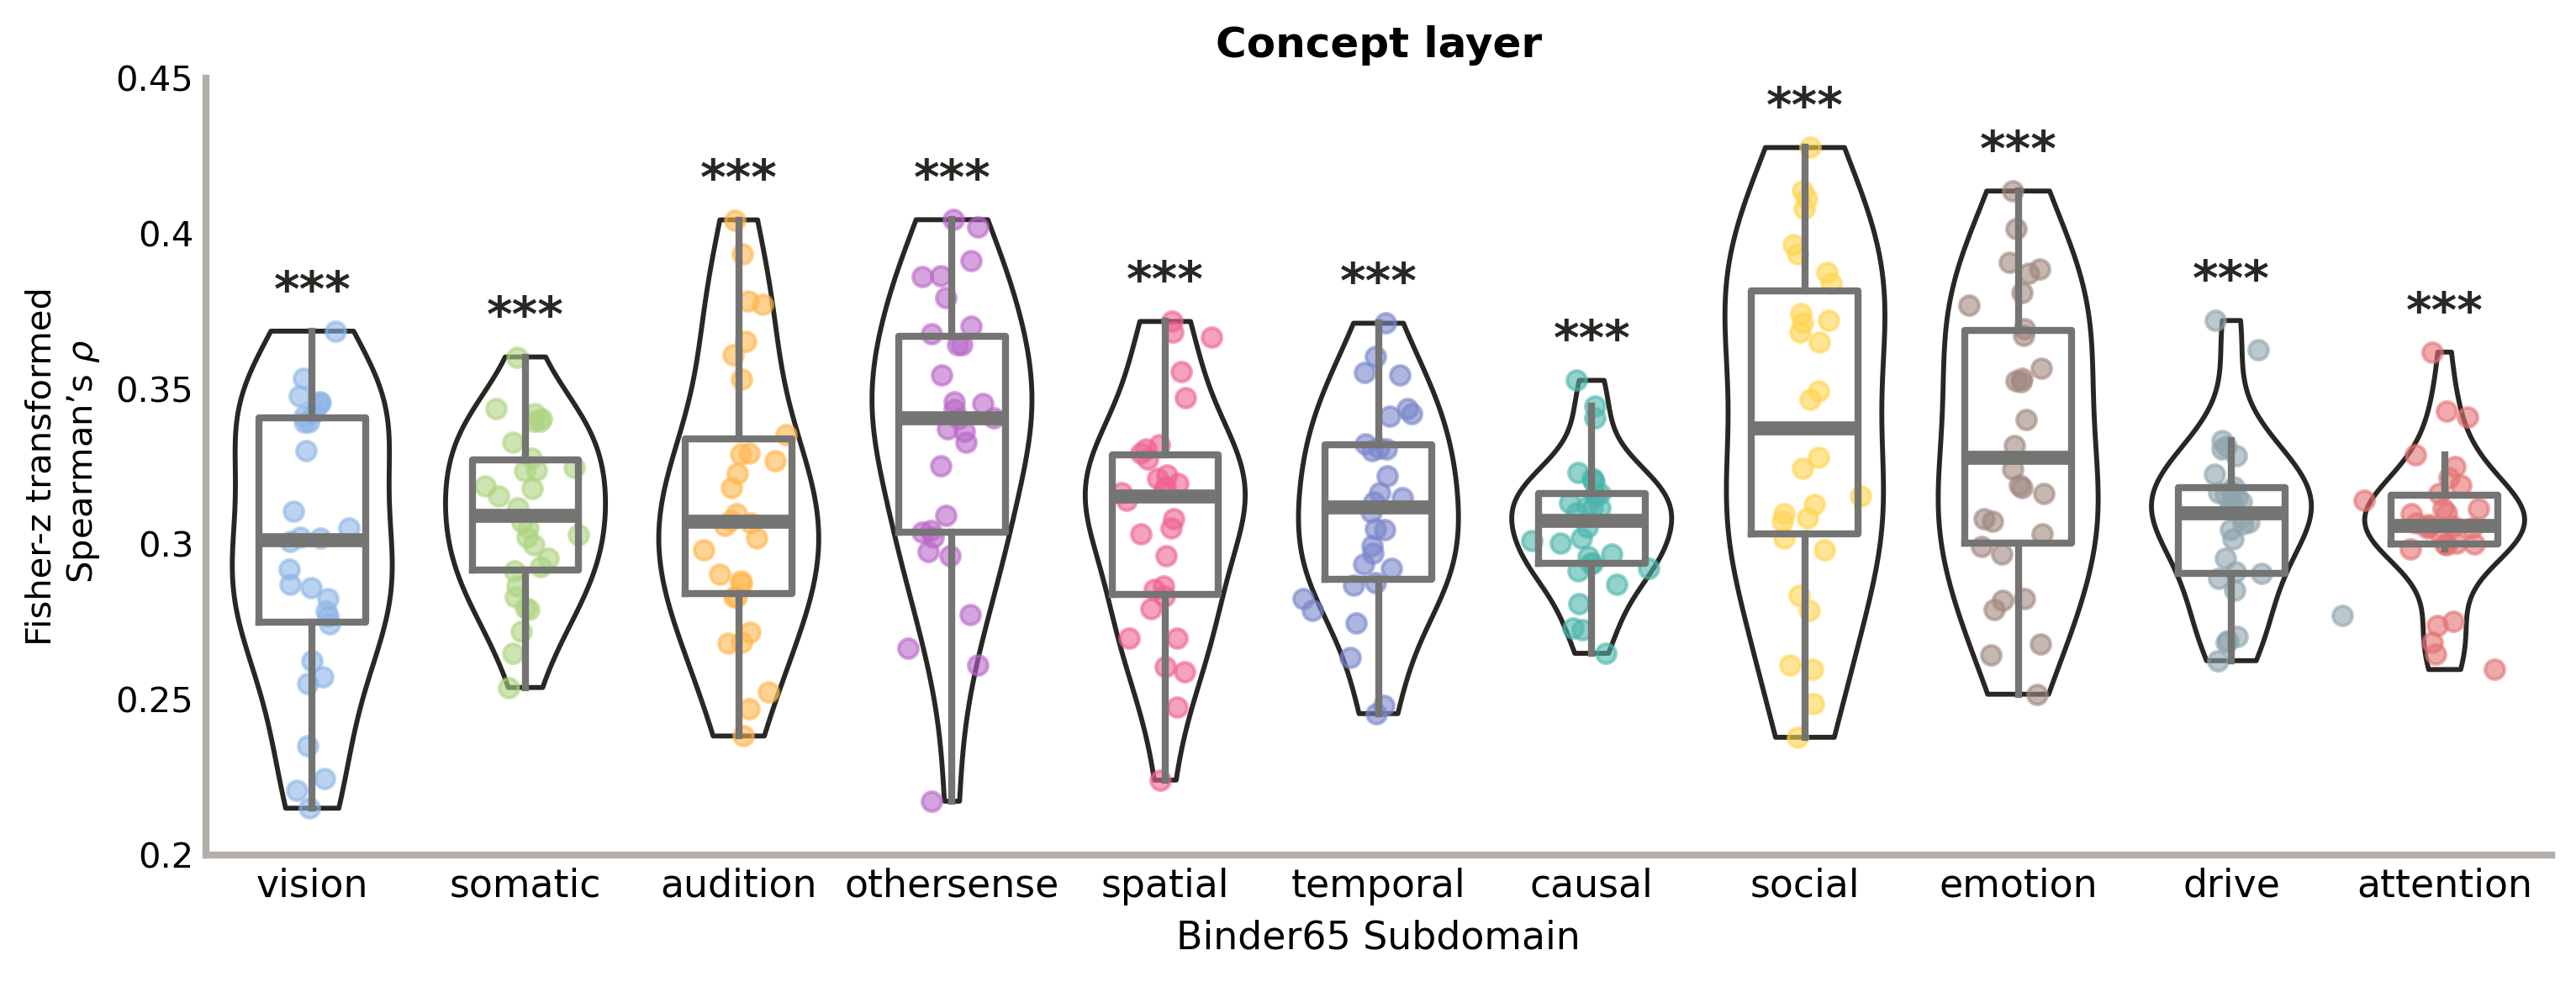
\includegraphics[width=0.9\textwidth]{fig/fig_s3.png}
\suppcaption{\textbf{$\vert$ Representational similarity between CATS concept layer and Binder65 subdomains.} This figure illustrates the RSA results between our CATS model's concept layer and the 11 subdomains of the Binder65 model. RDMs were generated for both the CATS concept layer and each Binder65 subdomain using WT95 stimulus dataset. The y-axis displays Fisher's \textit{z}-transformed Spearman’s rank correlation coefficients ($\rho$) between the respective RDMs. Violin plots show the distribution of these correlation values across 30 independently initialized CATS models, with embedded box plots indicating median and interquartile ranges. Individual data points represent correlation values from each independently trained model. Asterisks (***) above each subdomain indicate statistical significance ($p < 0.001$) from one-sample \textit{t}-tests conducted at the group level. The analysis reveals significant representational similarity between our CATS concept layer and all Binder65 subdomains, with particularly notable correlations observed in non-visual domains such as social and emotional processing domains.}
\label{figS3}
\end{figure}

\begin{figure}[htbp]
\centering
\includegraphics[width=0.9\textwidth]{fig/fig_s4.png}
\suppcaption{\textbf{$\vert$ Ablation studies and hyperparameter explorations.} The left most 2 bars was adopted from Fig~\ref{fig2}a, while the others represents the average of mean accuracy across 5 independently initialized models after training, and each point represents the corresponding mean accuracy cross all categories.}
\label{figS4}
\end{figure}

\begin{figure}[htbp]
\centering
\includegraphics[width=0.9\textwidth]{fig/fig_s5.png}
\suppcaption{\textbf{$\vert$ Ablation Studies on Concept Space Construction.} The left most one bar was adopted from Fig. 2a, while the others represents the average of mean accuracy across 5 independently initialized models after training, and each point represents the corresponding mean accuracy cross all categories.}
\label{figS5}
\end{figure}

% If your article has accompanying supplementary file/s please state so here. 

% Authors reporting data from electrophoretic gels and blots should supply the full unprocessed scans for key as part of their Supplementary information. This may be requested by the editorial team/s if it is missing.

% Please refer to Journal-level guidance for any specific requirements.

% \bmhead{Acknowledgements}

% Acknowledgements are not compulsory. Where included they should be brief. Grant or contribution numbers may be acknowledged.

% Please refer to Journal-level guidance for any specific requirements.

% \section*{Declarations}

% Some journals require declarations to be submitted in a standardised format. Please check the Instructions for Authors of the journal to which you are submitting to see if you need to complete this section. If yes, your manuscript must contain the following sections under the heading `Declarations':

% \begin{itemize}
% \item Funding
% \item Conflict of interest/Competing interests (check journal-specific guidelines for which heading to use)
% \item Ethics approval and consent to participate
% \item Consent for publication
% \item Data availability 
% \item Materials availability
% \item Code availability 
% \item Author contribution
% \end{itemize}

% \noindent
% If any of the sections are not relevant to your manuscript, please include the heading and write `Not applicable' for that section. 

% %%===================================================%%
% %% For presentation purpose, we have included        %%
% %% \bigskip command. Please ignore this.             %%
% %%===================================================%%
% \bigskip
% \begin{flushleft}%
% Editorial Policies for:

% \bigskip\noindent
% Springer journals and proceedings: \url{https://www.springer.com/gp/editorial-policies}

% \bigskip\noindent
% Nature Portfolio journals: \url{https://www.nature.com/nature-research/editorial-policies}

% \bigskip\noindent
% \textit{Scientific Reports}: \url{https://www.nature.com/srep/journal-policies/editorial-policies}

% \bigskip\noindent
% BMC journals: \url{https://www.biomedcentral.com/getpublished/editorial-policies}
% \end{flushleft}

% \begin{appendices}
% \section{Section title of first appendix}\label{secA1}


% An appendix contains supplementary information that is not an essential part of the text itself but which may be helpful in providing a more comprehensive understanding of the research problem or it is information that is too cumbersome to be included in the body of the paper.

% %%=============================================%%
% %% For submissions to Nature Portfolio Journals %%
% %% please use the heading ``Extended Data''.   %%
% %%=============================================%%

% %%=============================================================%%
% %% Sample for another appendix section			       %%
% %%=============================================================%%

% %% \section{Example of another appendix section}\label{secA2}%
% %% Appendices may be used for helpful, supporting or essential material that would otherwise 
% %% clutter, break up or be distracting to the text. Appendices can consist of sections, figures, 
% %% tables and equations etc.

% \end{appendices}

%%===========================================================================================%%
%% If you are submitting to one of the Nature Portfolio journals, using the eJP submission   %%
%% system, please include the references within the manuscript file itself. You may do this  %%
%% by copying the reference list from your .bbl file, paste it into the main manuscript .tex %%
%% file, and delete the associated \verb+\bibliography+ commands.                            %%
%%===========================================================================================%%

\clearpage

\bibliography{CA_TS_Net}% common bib file
%% if required, the content of .bbl file can be included here once bbl is generated
%%\input sn-article.bbl

\end{CJK}
\end{document}
